%rj2 4/7/19 Becomes second section in appendix after Simulation moved there.
%\section{Appendix - Alternatives}
%\label{appdx:fdsp-pd-alt}

\subsection{Options to Enhance Light Yield Uniformity}
\label{sec:fdsp-pd-enh}
%\metainfo

Due to a combination of geometric effects and the impact of Rayleigh scattering, the baseline \dword{sp} \dword{pds} design will result in non-uniformity of light collection along the drift direction. Light emitted from interactions close to the \dword{apa}s has an order of magnitude larger chance of being detected compared to interactions close to the \dword{cpa}.    

Though the designs described in the previous sections will meet the \dword{pd} performance requirements, %we have considered 
two options for enhancing both the light yield and light yield uniformity are under consideration.  Both approaches mitigate the impact of a short Rayleigh scattering length by converting \SI{127}{nm} scintillation photons to longer wavelength photons with a significantly longer Rayleigh scattering length. %A benefit of the 
An increase in uniformity %is that it 
will enhance the ability to do calorimetric reconstruction with scintillation light, %; this would 
thus enhancing the charge-based energy reconstruction %as well as 
and increasing the efficiency of triggering on low energy signals.

These options will be pursued in parallel with the baseline design and may be implemented after appropriate review if resources are available and if they do not interfere with, or produce unacceptable risk for, the baseline design schedule.


%>> Start: Andrzej Szelc 14/02/2018 >>>>>>>>>>>>> 
% Not a publication, but a proceedings:  To cite this article: Diego Garcia-Gamez and SBND Collaboration 2017 J. Phys.: Conf. Ser. 888 012094

\subsubsection{Coated Reflector Foils on the TPC Cathode}
\label{sec:fdsp-pd-enh-cathode}

%\fixme{ETTORE:  DIEGO REQUESES OUR MOTIVATION FOR COATING THE CATHODE RATHER THAN THE FIELD CAGE (Like the DP PD)}
%Ettore: fixed

In this option, scintillation light falling on the cathode plane is converted into the visible wavelengths and reflected.
Installing the foils on the cathode represents the option  with the minimal impact on the current design of the HV system (field cage and cathode) and ensures a good uniformity of the light yield across the detector.
This light could then be detected by the \dwords{pd} embedded in the \dword{apa}, improving the overall collection efficiency. This option would require at least a fraction of the light collectors be sensitive to visible light. This sensitivity to visible light can be achieved in two ways: (1) by coating the \dword{xarapu} with TPB instead of \dword{ptp}, which results in the same WLS combination as the double shift bars (whose performance is measured in \dword{pdsp})
and/or (2) by leaving some of the \dword{xarapu} detectors without a  
WLS coating and with an appropriate dichroic filter. In the former case the \dwords{pd}  are sensitive to both the direct and reflected light, in the latter case only to the reflected light. 

Figure~\ref{fig:ly_with_foils} shows the simulated results of a configuration where 50\% of the \dword{apa} light collectors can %are capable of recording 
record both direct scintillation light and the reflected visible light from the \dword{cpa},  and 50\% are left uncoated to maximize uniformity. This results in an enhancement of the total light collection close to the cathode (black points). %, which will increase the detection efficiency in that region. (sounds redundant. anne)

Introducing the foils on the cathode may also enable drift position resolution using only scintillation light. This requires the \dwords{pd} to  
differentiate direct \dword{vuv} light from re-emitted visible light (i.e., requires two 
types of \dword{pd}) and 
sufficient timing of arrival of first light.

Coated reflector foils are manufactured through low-temperature evaporation of \dword{tpb} on dielectric reflectors e.g. 3M DM2000 or Vikuiti  ESR. Foils prepared in this manner have been successfully used in dark matter detectors such as WArP~\cite{Acciarri:2008kv}. Recently they have been shown to work in \dwords{lartpc} at neutrino energies, namely  in the LArIAT test-beam detector~\cite{Garcia-Gamez:2017cmu}. In \dword{lariat} they have been installed on the field-cage walls and, during the last run, on the cathode. An alternative solution would be to use Polyethylene Naphthalate (PEN) instead of TPB. This wavelength-shifter has a similar emission spectrum to TPB \cite{Kuzniak:2018dcf}, but is provided in sheets, which could greatly simplify the production and installation. The choice of using PEN depends on demonstrating that its performance holds in \lar\ -- these studies are ongoing. 
%The necessity to record both \dword{vuv} and visible photons in the light collectors would require a change in the current design but is conceptually possible. For example, if the cathode plane were coated with tTP,  some of the ARAPUCA modules could be constructed without the pTP coating on the outer surface of the filter and benefit from the same photon trapping effect but these cells would no longer be sensitive to direct scintillator light.   
%Understanding the impact of these competing effects on the physics is under study by the simulation group and
The method of foil installation is being developed in collaboration with the DUNE HV consortium, with the objective of minimizing the impact on the \dword{cpa} design. 

%A run has been performed using the CERN FLIC 50l prototype TPC, with
%the DUNE-like resistive cathode covered with a non-perforated DM2000
%foil evaporated with TPB. No obvious HV problems were observed, however
%the data is still being analyzed to understand whether any field
%distortions were present.  
% rjw The following commented out pending update from Andrzej.
%Another run with the cathode coated with PEN is scheduled for January/February 2019.
%\fixme{Request in to Andrzej to update this previous paragraph.}

%\fixme{Andrzej: results of this test should be ready for tdr; rjw what is the schedule for this?   Email sent to Andrzej 1/12/19}
%In particular, the feasibility of coating the cathode with a dielectric medium is being investigated - the current solution is to prepare the foil plates with small perforations which would allow the electric field lines to safely neutralize on the \dword{cpa} underneath. A dedicated R\&D test is being performed at CERN using the ICARUS 50l with a TPB evaporated foil on the \dword{cpa}. 

%Update from Andrzej 4/21/19
A run has been performed using the CERN FLIC \SI{50}{l} prototype TPC, with
the DUNE-like resistive cathode covered with a non-perforated DM2000
foil evaporated with TPB. No obvious high-voltage problems were observed, however
the data is still being analyzed to understand whether any field
distortions were present.  A second run with the cathode coated with PEN
was performed in March 2019. The comparison of effects on the electric field between the two solutions is in progress, preliminary studies show that PEN seems to work as a wavelength-shifter at liquid argon temperatures, but may not be as efficient as TPB. A future run will involve running with a perforated TPB coated foil. The presence of the holes maintains the resistive character of the cathode and minimizes the effect of electric field distortions. 

%\fixme{ETTORE--  DIEGO REQUESTS MOTIVATION FOR PERFORATED FOIL.  "I miss a line here motivating the test with perforated TPB coated foil."}
%fixed

\begin{dunefigure}[Predicted light yield with WLS-coated reflector foils on the CPA]{fig:ly_with_foils}
{Predicted light yield in the \dword{pds} with WLS-coated reflector foils on the \dword{cpa}. Blue points represent direct \dword{vuv} light impinging on the \dwords{pd} assuming a 2.5\% photon detection efficiency and 70\% wire mesh transmission and half of the detectors left uncoated; red stars - represent scintillation light that has been wavelength-shifted and reflected on the \dword{cpa} assuming the same photon detection efficiency folded in with an 80\% transmittance of the filters to visible light. Black points show the sum of these two contributions.}
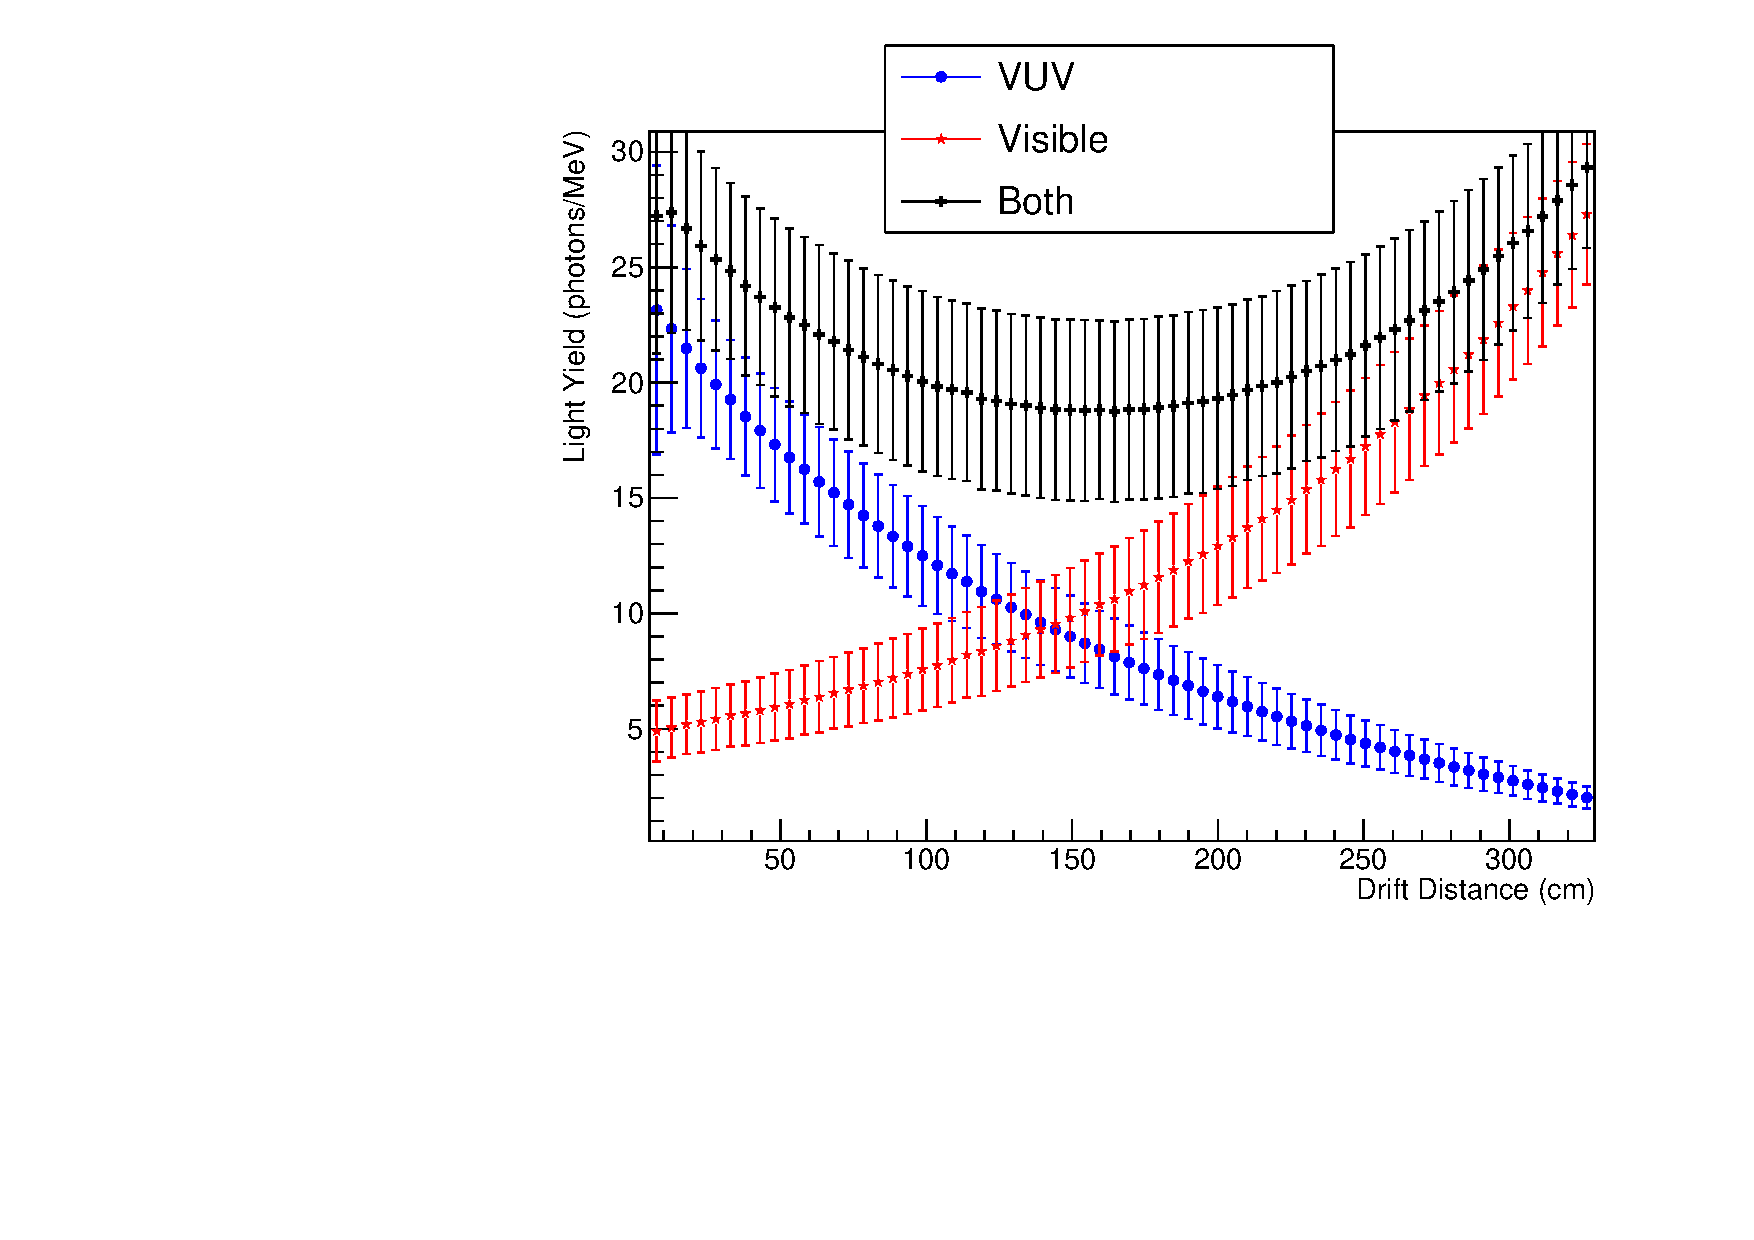
\includegraphics[width=0.5\columnwidth]{pds-ly_with_foils_new.pdf}
\end{dunefigure}

\subsubsection{Doping Liquid Argon with Trace Parts of Xenon}
\label{sec:fdsp-pd-enh-xenon}
%text edited by rjw 

%The main motivation for this proposed option is to overcome the serious reduction in the response of the photon detection (PD) system to events  as they occur further from the light collectors (PC), towards the TPC cathode (\dword{cpa}). Improving the response across the TPC volume will both increase the trigger efficiency and simplify the analysis for supernova neutrinos. An increased response would also be beneficial for the determination of t0 for nucleon decay events. 
%\fixme{174, 175 or 176 nm?}

This option exploits the conversion of the LAr \SI{127}{nm} light to \SI{175}{nm} by doping the \lar volume with 20-100 ppm of xenon.  While there are indications that the absolute light yield in xenon-doped argon may be higher than in pure argon, in the current estimates we assume the yields are the same. In this case, the source of the improved performance described here is the much longer Rayleigh scattering length for \SI{175}{nm} light.  The improvement is illustrated in Figure~\ref{fig:visibility_with_xenon} from a DUNE \dword{pd} simulation, assuming an absorption length for the scintillation light of \SI{20}{m}. The gain in average yield for events near the \dword{cpa} is about a factor five.

\begin{dunefigure}[Simulation of \lar scintillation light with and without Xe doping in a \dshort{spmod}]
{fig:visibility_with_xenon}
{Simulation of visibility of \SI{128}{nm} (LAr with xenon doping) and \SI{176}{nm} (LAr scintillation) light in a \dword{sp} module.}
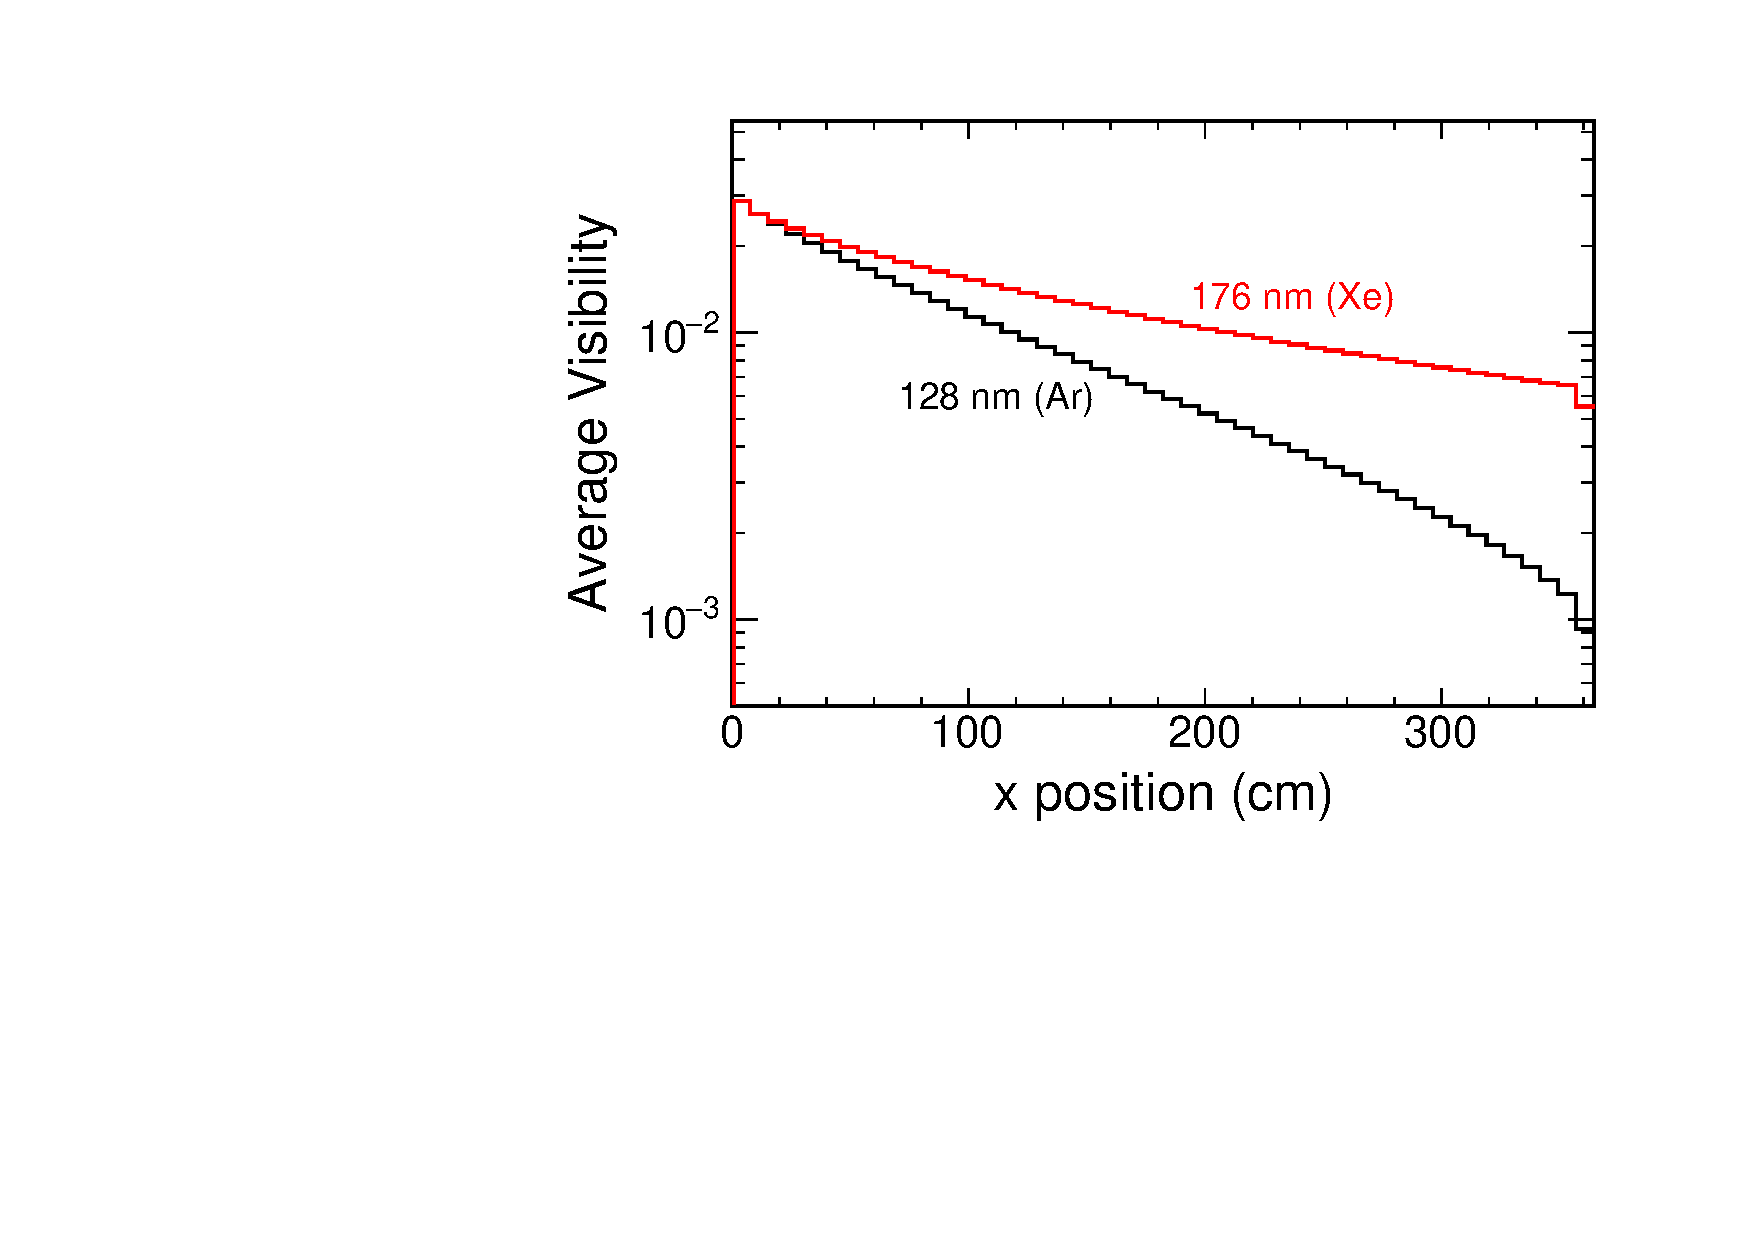
\includegraphics[width=0.5\columnwidth]{pds-ly_with_xenon.pdf}
\end{dunefigure}

Doping with xenon also affects the time structure of the scintillation light and in particular reduces the fraction of late light.  Having a light signal of shorter duration can bring advantages both in physics, such as making it easier to tag Michel electrons from pions and electrons, and in the electronics required. The longer wavelength of the scintillation light resulting from the Xe doping allows the possibility of simplifying the design of the \dword{pds} light collectors (\dword{xarapu}) by dispensing with the use of the outer layer of wavelength shifting material, thereby reducing costs and simplifying the handling of the light collectors during storage and installation. 

%{\it \bf  Implementation and rough cost}

%The diagram in Figure~\ref{fig:cryo_with_xenon} is a schematic of the argon delivery and recirculation system for DUNE.  
Doping the argon with xenon is facilitated by the fact that at the DUNE Far Detector the argon is transported from the surface to underground as gas before it is re-condensed for delivery to the cryostats. Xenon and argon can therefore be mixed in gas form before condensation;  in consultation with the cryogenic experts, we have identified locations where this mix could be achieved. Since the operations take place at room temperature, the implementation is relatively straightforward.
%the diagram shows locations where this mix could be achieved. Since the operations take place at room temperature, the implementation is relatively straightforward.

%\begin{dunefigure}[Schematic of the argon delivery and recirculation system for DUNE indicating possible locations for argon and xenon premixing.]{fig:cryo_with_xenon}
%{Schematic of the argon delivery and recirculation system for DUNE indicating possible locations for argon and xenon premixing.}
%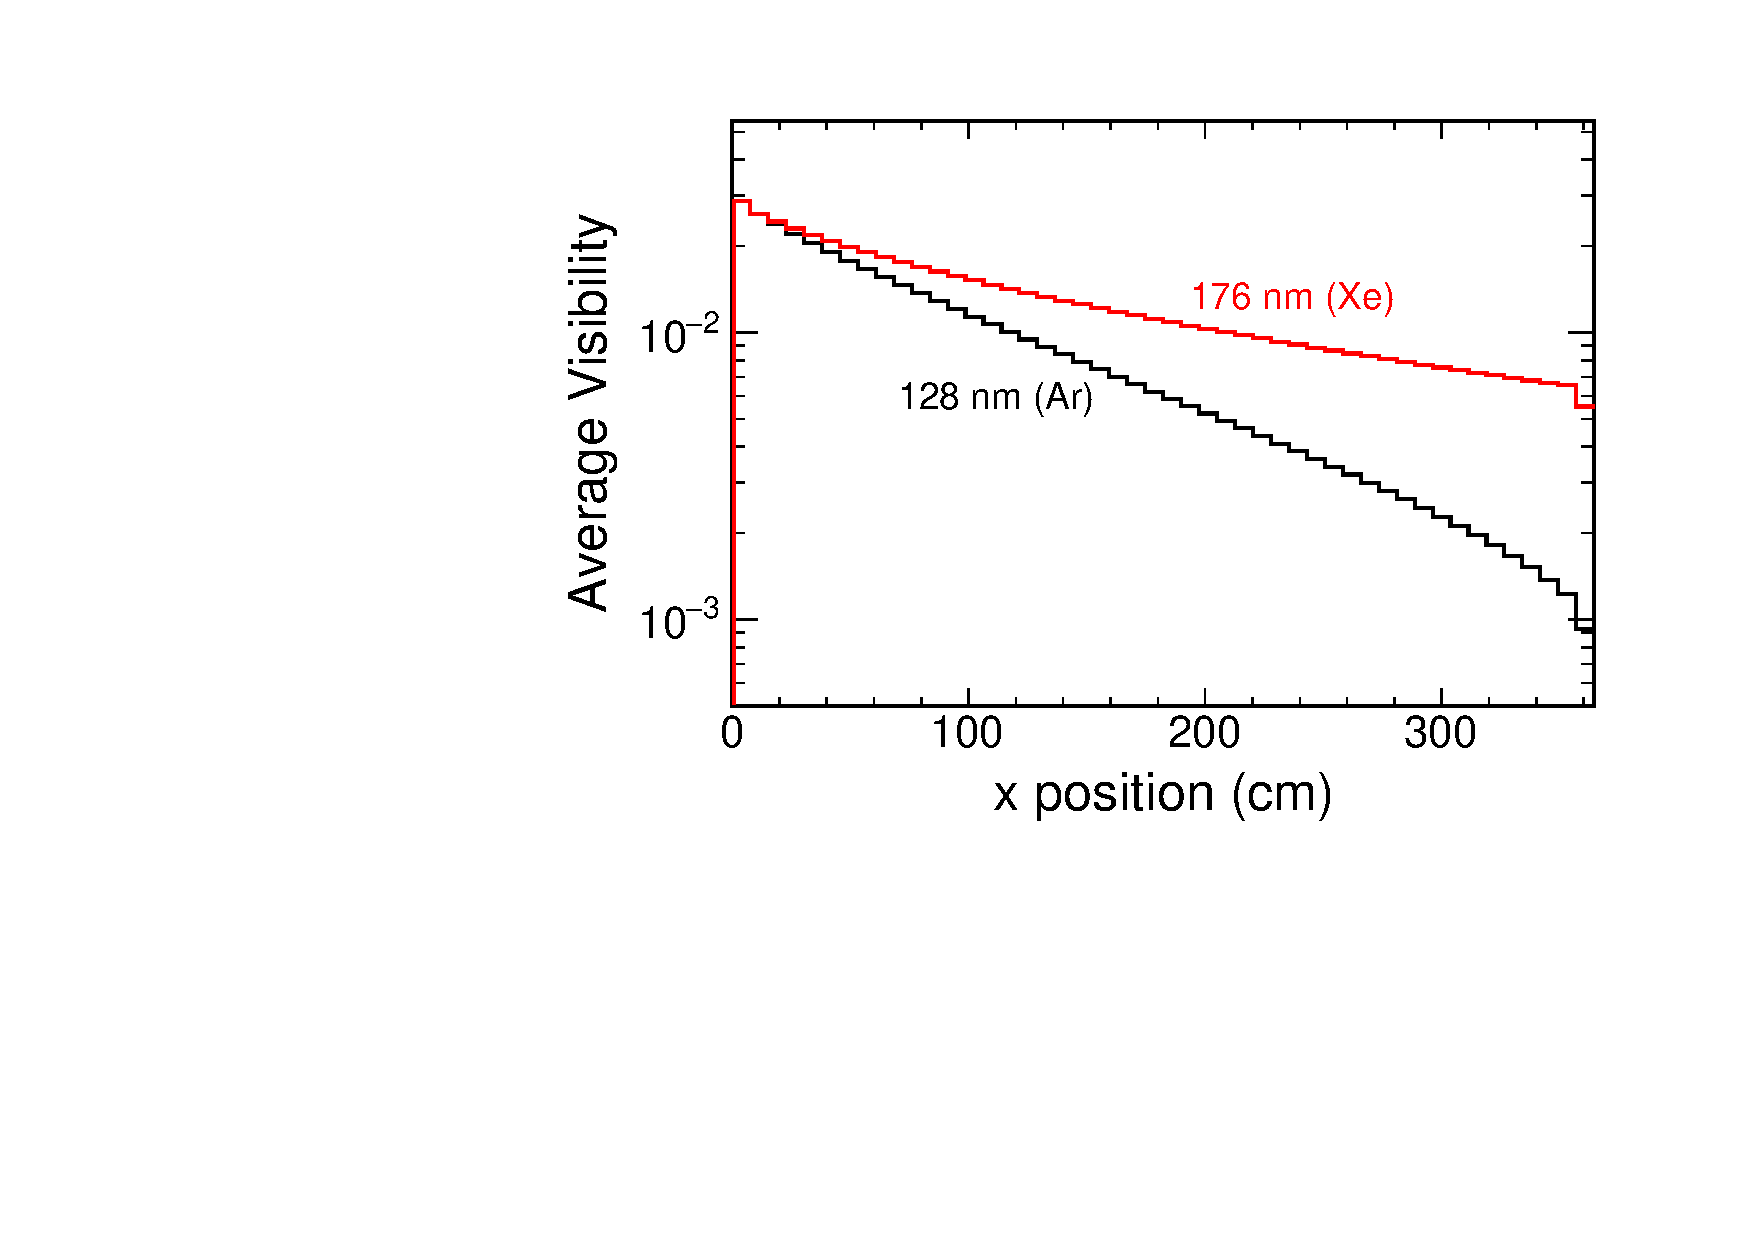
\includegraphics[width=0.6\columnwidth]{pds-ly_with_xenon.pdf}
%\end{dunefigure}

%A detailed cost estimate will require an evaluation of flow rates, piping design, etc. The major cost is expected to be the xenon, which would be ~ \$20,000/(ppm Xe doping) per Far Detector module. The physics results outlined above can be achieved for doping levels between 20 to 100 ppm of xenon.

{\it\bf Critical Issues and R\&D Work}

Xenon doping must not adversely affect the performance of the TPC and while the doping is expected to be neutral or even beneficial, its effects on charge yield, drift lifetime and HV stability need to be established.  There is experience in xenon doping of argon both at CERN and Fermilab, and tests for the TPC effects are being designed.  
More detailed R\&D is needed to optimize the xenon doping fraction and its interaction with the light-detection system. This can be conducted on a time scale of about a year by a small number of dedicated investigators using resources that, mostly, are expected to be available at Fermilab and CERN. 

%%%%%%%%%%%%%%%%%%%%%%%%%%%%%%%%%%%%%%%%%%%%%%%%%%%%%%%%%%%%%%%%%%%%%%%%%%%%%%%%%%%%%%%%%%%%%